% Primary source: https://arxiv.org/abs/1703.06103
\documentclass[tikz,border=5pt]{standalone}
\usepackage[T1]{fontenc}
\usepackage{lmodern,amsmath,amssymb}
\usetikzlibrary{arrows.meta,calc,positioning,fit,backgrounds,shapes.geometric,matrix,decorations.pathreplacing,patterns}
\definecolor{ink}{gray}{0.08}
\definecolor{wash}{gray}{0.965}
\definecolor{soft}{gray}{0.45}
\tikzset{box/.style={draw=ink,line width=.65pt,fill=white,align=center,inner sep=4pt,outer sep=0pt,font=\small},flow/.style={draw=ink,line width=.65pt,-{Latex[length=1.8mm,width=1.3mm]},rounded corners=2pt},annotation/.style={font=\scriptsize,text=soft,align=center},groupbox/.style={draw=soft,dashed,line width=.45pt,fill=wash}}
\begin{document}
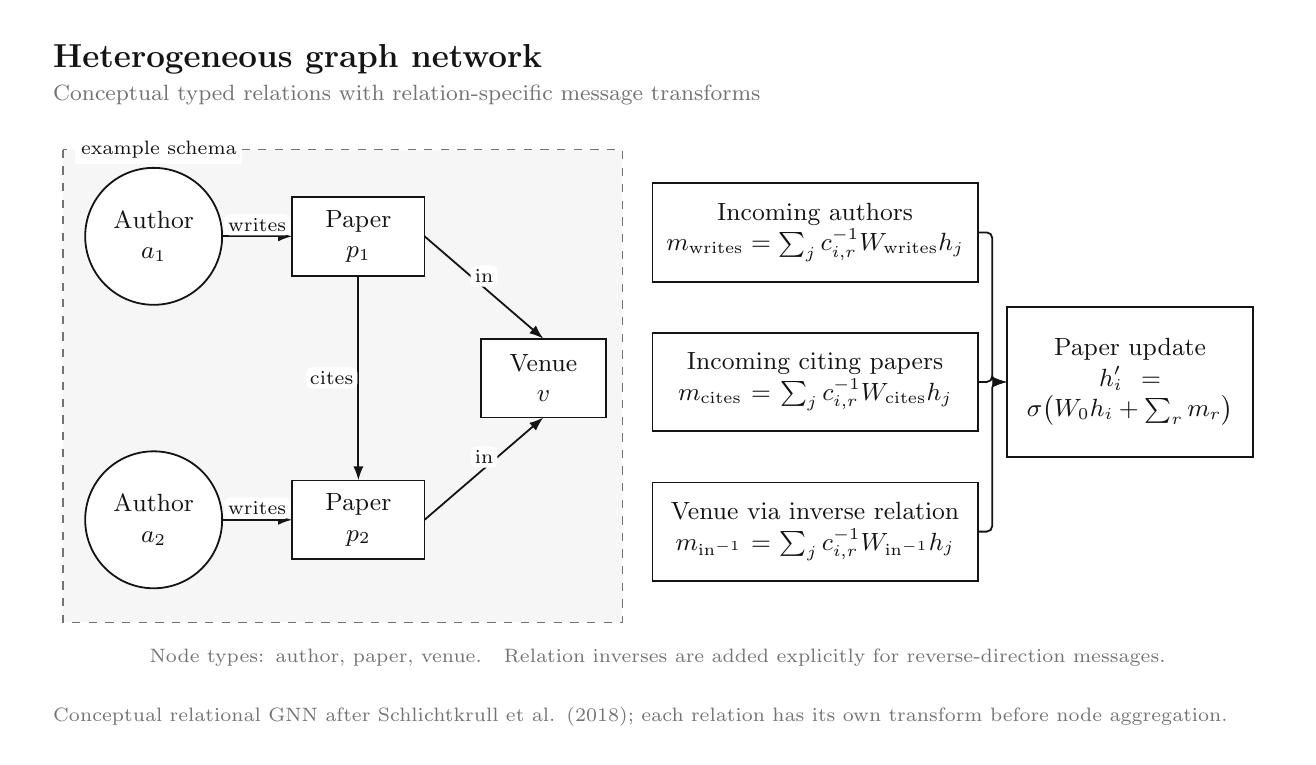
\begin{tikzpicture}[x=1cm,y=-1cm,font=\rmfamily,text=ink]

\path[use as bounding box] (0,0) rectangle (16,9);
\node[anchor=west,font=\large\bfseries] at (.2,.4) {Heterogeneous graph network};
\node[anchor=west,font=\footnotesize,text=soft] at (.2,.85) {Conceptual typed relations with relation-specific message transforms};
\begin{pgfonlayer}{background}
\draw[groupbox] (0.45,1.55) rectangle (7.55,7.55);
\node[anchor=west,font=\scriptsize,fill=white,inner sep=2pt] at (0.6,1.55) {example schema};
\end{pgfonlayer}
\node[box,circle,minimum width=1.45cm,minimum height=1.0cm,text width=1.2cm] (a1) at (1.6,2.65) {Author\\$a_1$};
\node[box,circle,minimum width=1.45cm,minimum height=1.0cm,text width=1.2cm] (a2) at (1.6,6.25) {Author\\$a_2$};
\node[box,minimum width=1.65cm,minimum height=1.0cm,text width=1.4cm] (p1) at (4.2,2.65) {Paper\\$p_1$};
\node[box,minimum width=1.65cm,minimum height=1.0cm,text width=1.4cm] (p2) at (4.2,6.25) {Paper\\$p_2$};
\node[box,minimum width=1.55cm,minimum height=1.0cm,text width=1.3cm] (venue) at (6.55,4.45) {Venue\\$v$};
\node[box,minimum width=4.1cm,minimum height=1.25cm,text width=3.8499999999999996cm] (writes) at (10.0,2.6) {Incoming authors\\$m_{\rm writes}=\sum_j c_{i,r}^{-1}W_{\rm writes}h_j$};
\node[box,minimum width=4.1cm,minimum height=1.25cm,text width=3.8499999999999996cm] (cites) at (10.0,4.5) {Incoming citing papers\\$m_{\rm cites}=\sum_j c_{i,r}^{-1}W_{\rm cites}h_j$};
\node[box,minimum width=4.1cm,minimum height=1.25cm,text width=3.8499999999999996cm] (inv) at (10.0,6.4) {Venue via inverse relation\\$m_{{\rm in}^{-1}}=\sum_j c_{i,r}^{-1}W_{{\rm in}^{-1}}h_j$};
\node[box,minimum width=3.1cm,minimum height=1.9cm,text width=2.85cm] (update) at (14.0,4.5) {Paper update\\$h'_i=\sigma\!\left(W_0h_i+\sum_r m_r\right)$};
\begin{pgfonlayer}{background}
\draw[flow] (a1.east) -- (p1.west) node[midway,above,fill=white,inner sep=1.5pt,font=\scriptsize] {writes};
\draw[flow] (a2.east) -- (p2.west) node[midway,above,fill=white,inner sep=1.5pt,font=\scriptsize] {writes};
\draw[flow] (p1.south) -- (p2.north) node[midway,left,fill=white,inner sep=1.5pt,font=\scriptsize] {cites};
\draw[flow] (p1.east) -- (venue.north) node[midway,above,fill=white,inner sep=1.5pt,font=\scriptsize] {in};
\draw[flow] (p2.east) -- (venue.south) node[midway,above,fill=white,inner sep=1.5pt,font=\scriptsize] {in};
\draw[flow] (writes.east) -- (12.25,2.6) -- (12.25,4.5) -- (update.west);
\draw[flow] (cites.east) -- (12.25,4.5) -- (12.25,4.5) -- (update.west);
\draw[flow] (inv.east) -- (12.25,6.4) -- (12.25,4.5) -- (update.west);
\end{pgfonlayer}
\node[annotation,text width=14.2cm] at (8.0,8.0) {Node types: author, paper, venue.\quad Relation inverses are added explicitly for reverse-direction messages.};
\node[anchor=west,align=left,font=\scriptsize,text=soft,text width=15.6cm] at (.2,8.75) {Conceptual relational GNN after Schlichtkrull et al. (2018); each relation has its own transform before node aggregation.};
\end{tikzpicture}
\end{document}
